\textbf{COLUNI 2024 -- Questão 24}\par\medskip A figura abaixo apresenta duas lâmpadas, uma incandescente ($L_1$) e outra de LED ($L_2$), de potências iguais a 60 W e 9 W, respectivamente. O fabricante afirma que ambas apresentam a mesma luminosidade.

\begin{center}
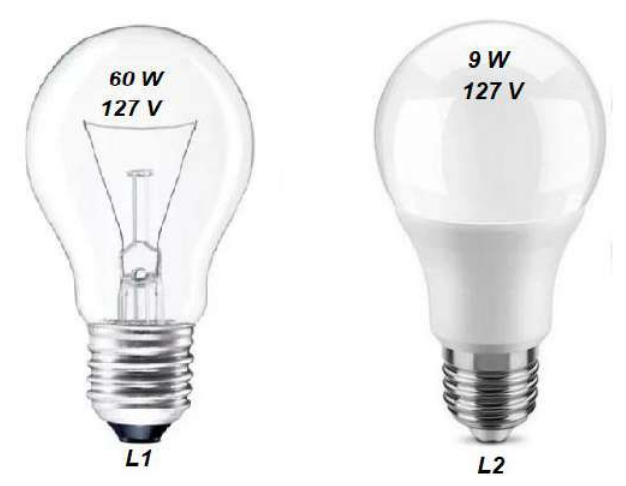
\includegraphics[width=0.52\linewidth]{static/simulados/coluni/figuras/2024/questao-24/figura-1.png}
\end{center}

Sabendo-se que a potência de um aparelho representa a quantidade de energia consumida por tempo e, considerando que as lâmpadas ficam acesas 5 horas por dia, é CORRETO afirmar que, ao substituirmos a lâmpada incandescente pela lâmpada de LED, a economia mensal de energia elétrica, em quilowatt-hora (KWh), será de:
\begin{enumerate}
\item 1,35
\item 5,10
\item 7,65
\item 9,00
\end{enumerate}
